\begin{figure}[H]
	\centering
	\resizebox{100mm}{!}{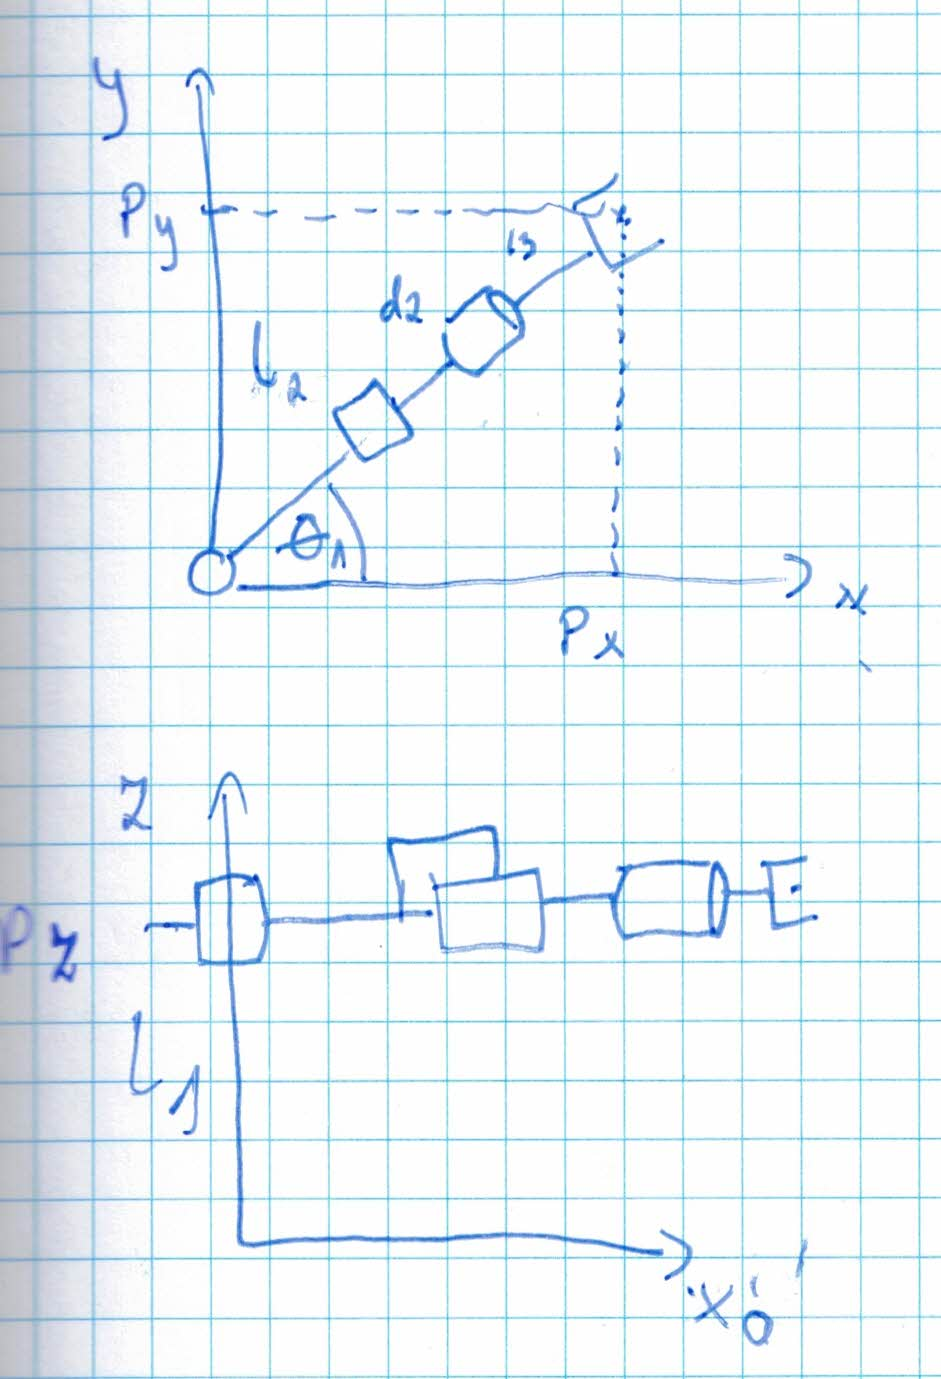
\includegraphics{src/odwrotna_2.jpg}}
	\caption{Widok z góry i boku robota wykorzystane podczas obliczania kinematyki odwrotnej} 
\end{figure}    

\begin{figure}[H]
\centering

$q=
\begin{bmatrix}
\theta _1 \\
d_2 \\
\theta_3 \\
\end{bmatrix}  
=
\begin{bmatrix}
atan2(cos(\sqrt{p_x^2+p_y^2},sin(\sqrt{p_x^2+p_y^2}))\\
\sqrt{p_x^2+p_y^2}-l_2-l_3\\
\theta_3 \\
\end{bmatrix}  $


\caption{Macierz transformacji robota} 
\end{figure} 
$ \theta_3$ nie wpływa na zmianę położenia końcówki (jedynie na jej orientację względem układu bazowego). 